\chapter[Application]{Application to manual wheelchair locomotion}
\label{application}
\section{Introduction}
The moment of a force around an axis is a physical vector quantity, which measures the ability of the force to rotate a solid around an axis. In the case of wheelchair locomotion, the moment measures a subject's ability to turn the wheels of his Wheelchair, that is, to move with his Wheelchair. It is, therefore, a quantity whose measurement is essential for the analysis of locomotion in a Manual Wheelchair. With this in mind, a sensor capable of measuring wheel moment was installed on the field-ergometer manual wheelchair.  In this chapter, we will analyse the measurements made by this sensor to understand manual wheelchair locomotion better. To do this, we will first present the moment-sensor, then the data sets that are the subject of our analyses. We will then revisit the classic questions of manual wheelchair locomotion: the symmetry of manual wheelchair locomotion, the evaluation of the propulsion capacities of subjects in manual wheelchairs.

\section{The torsor sensor}

A torsor is a mathematical object used to characterize the movements of a solid. It measures both the forces and moments applied to this object along three axes. A torsor sensor was designed, built and installed on the wheels of the field-ergometer manual wheelchair (Fig. \ref{capteur_tri_axe}), to measure the forces exerted by wheelchair users during their locomotion.

\begin{figure}[h]
\center
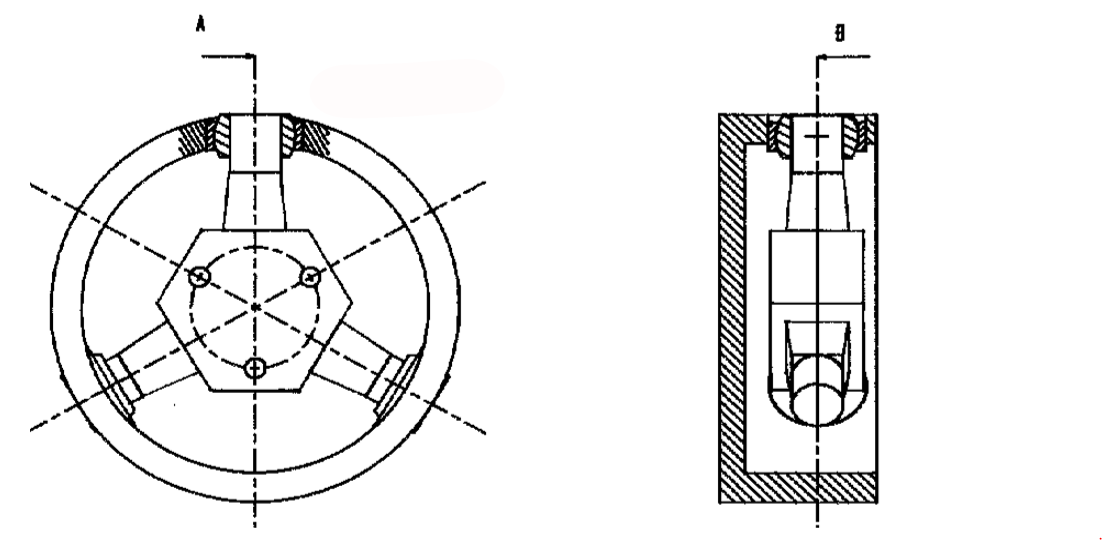
\includegraphics[scale = 0.4]{images/capteur_tri_axe}
\caption{Torsor sensor, brevet WO 1995001556 A1}
\label{capteur_tri_axe}
\end{figure}

It consists of three bidirectional sensors measuring the forces applied to the handrail.

\section{Description of  datasets}
The data sets we use throughout these tests are from experiments that were conducted with subjects with disabilities; here, the measurements were intended to understand manual wheelchair locomotion and also to evaluate the mechanical stresses it exerts on manual wheelchair users. In the other case, experiments were conducted with valid subjects. Here, the objective was to measure the impact of the experience on the propulsion technique used by the subjects. 


In both cases, the measurements made produce noisy, cyclic and uncertain time series (Fig. \ref{TWMWC}). All subsequent treatments are performed on the Z moment measured on the wheels of a manual wheelchair field ergometer.

\begin{figure}[h]
\center
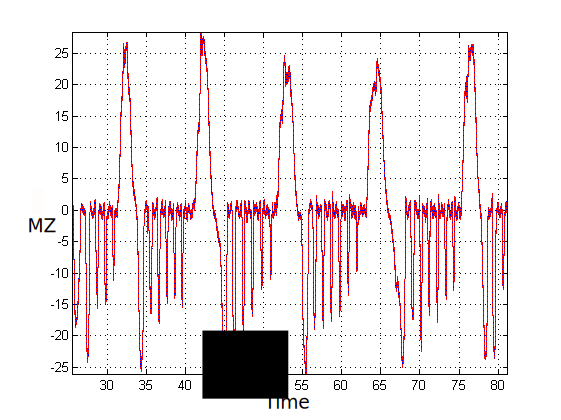
\includegraphics[scale = 0.5]{images/TSMWC}
\caption{Example of Z moment from a wheel of a  field-ergometer manual wheelchair}
\label{TWMWC}
\end{figure}


We want to return to the characteristic properties of the Z moments measured by the torsor sensor and explain why the recorded measurements are long, noisy, cyclic and uncertain.

\paragraph{Length of time series:} the length of the time series is due to the high acquisition frequency of the torsor sensor. The acquisition frequency is 100Hz in other words; the sensor makes 100 measurements per second. Thus, a 10-minute recording generates a time series of $100 \times 60 \times 10 = 60,000$ data points. As another example is the Z moment of the left wheel of subject S02 has $107 227$ data points (Fig. \ref{mz_left_wheel}). The length of time series is problematic because the processing time of time series is highly dependent on their length. As an illustration, the time complexity of comparing two time series using the DTW alignment algorithm is $O(n^2)$ where $n$ is the length of the time series.

\begin{figure}[h]
\center
\includegraphics[scale = 0.6]{images/mz_left_wheel}
\caption{Z moment of the left wheel of manuel wheelchair recorded during the locomotion of subject S02}
\label{mz_left_wheel}
\end{figure}


\paragraph{Noise in time series:} The time series noise comes from the sensitivity of the torsor sensor which measures low-intensity forces applied to the handrail during manual wheelchair locomotion. These forces can come from the texture of the ground, the friction of the arm on the handrail during the movement or other. Noise in time series is problematic because it influences the calculation of the distance between two time-series, the division into cycles of a cyclic time series, or even the computation of properties that can characterize a time series.

\begin{figure}[h]
\center
\includegraphics[scale = 0.5]{images/TSN}
\caption{Time series recorded by torsor sensor are noisy}
\label{TWMWC}
\end{figure}

\paragraph{Cycles in time series:} The cyclical aspect of the time series comes from the cyclical nature of the movement in the Manual Wheelchair. Indeed, manual wheelchair movement consists of a succession of push moments during which the user of the manual wheelchair applies a force on the handrail of the wheelchair to move it and freewheel moment, instant during which the user of the manual wheelchair rests and takes momentum for the next push. The push is recorded by the sensor and materialized by a peak in the measurements, the periods of freewheel correspond to the values close to zero(Fig. \ref{TWMWC}). 

\paragraph{Uncertainty in time series :} The presence of uncertainty in sensor measurements is not a myth; it is a reality. To realize it, it is necessary to first understand the calibration process of the sensors in general, and of the torsor sensor in the case of this work. 
There are two leading families of sensors: piezo-resistive and piezo-electric, that have a similar operating principle. When a force is applied to the sensor, it causes a deformation of the sensor which induces a change in its resistance in the case of the piezo-resistive sensor or a change in the electrical voltage at its terminals, as is the case with piezoelectric sensors. The functioning of the sensor is based on the assumption that the change in resistance or electrical voltage induced by the force is proportional to the intensity of the force. Thus, the  sensor measures variation in resistance or electrical voltage and uses the proportionality relationship to infer the intensity of the force that has been applied. Calibrating a sensor consists in constructing this proportionality relation by applying greater and greater or smaller and smaller forces on the sensor. Doing so, we record a sequence of couples of force intensity, electrical voltage (or resistance) which is used to plot a regression line which will then be used to deduct the applied force knowing the voltage intensity  variation. However, the regression line does not define a perfect proportionality relationship. In fact, it minimizes the error made but does not cancel it. This error (Fig. \ref{residus}) introduces uncertainty into the estimation of the applied force intensity. It is essential to take this error into account when processing time series to extract relevant information from them.
Characterization of uncertainty is a time-consuming task (Appendix .\ref{pdf_uncertainty}) and is not always possible because sensor calibration data are generally not available. We, therefore, chose during these experiments to consider strategies that did not require knowledge of the probability distribution of uncertainty.

\begin{figure}[h]
\center
\includegraphics[scale = 0.5]{images/residus}
\caption{Residus of Mz; they represents difference between the real value and the value measured by the sensor.}
\label{residus}
\end{figure}

We will then explain how we use this data for the analysis of Manual Wheelchair locomotion. We remove noise on time series using a moving average filter. However, we don’t compress the time series using FDTW because we don’t have classes labels. 

\section{Manual Wheelchair locomotion analysis}

\subsection{Preprocessing}
Removing the noise contained in the time series and reducing their length are prerequisites to its operation for the analysis of manual wheelchair locomotion.

\subsection{Exploitation of time series of rolling chair locomotion}

\subsubsection{The symmetry of Manual Wheelchair Locomotion}
For a long time, experts assumed that the Manual Wheelchair locomotion was symmetrical, which made it possible to construct measuring instruments consisting of a single wheel \cite{brouha1967continuous}. Subsequently, the conclusions that were drawn from the measurements made with one wheel were generalized to both upper limbs of the subject. Then \cite{langbein1993research} built a roller ergometer capable of separately measuring the speed and resistance of the left and right wheels of the Manual Wheelchair during its use. The measurements taken from this roller ergometer revealed a difference between the properties measured by the left and right wheels and allowed the asymmetric character of the Manual Wheelchair locomotion to be deduced. In this paragraph, we use the SAX-P symbolic representation and the additional information we have on the subjects to carry out a new analysis of the symmetry of manual wheelchair locomotion.


As we have already demonstrated in chapter \ref{chapter_saxp}, even if a user of a Manual Wheelchair makes the same number of pushes with the right and left wheels during a straight line movement, these cycles may have different properties, which in our case takes the form of different letters in the character strings corresponding to the right and left wheels. This asymmetry of the locomotion in the Manual Wheelchair can be evaluated by calculating a relative Edit distance between the characters strings that correspond to the straight line displacements of the of the right and left wheels. The relative Edit distance counts the number of different letters between two characters strings.

\[
D(X,Y)=\frac{1}{n}\stackrel[i=1]{n}{\sum}[X_{i}\neq Y_{i}]
\]









\begin{longtable}
   {|p{0.35\linewidth}|p{0.2\linewidth}|p{0.1\linewidth}|}
   
   \hline
\multicolumn{1}{|l|}{\textbf{Subject}} & \multicolumn{1}{|l|}{\textbf{Straight displacement}} & \multicolumn{1}{|l|}{\textbf{Relative Edit Distance}}\endfirsthead 
 \hline

\multicolumn{1}{|l|}{\textbf{Subject}} & \multicolumn{1}{|l|}{\textbf{Straight displacement}} & \multicolumn{1}{|l|}{\textbf{Relative Edit Distance}}  \\

	 \hline
   \multicolumn{3}{|p{0.65\linewidth}|}{Following ... } \\

   \hline
	 \endhead

   \hline
   \multicolumn{3}{|p{0.65\linewidth}|}{Continue to the next page}\\ 

	 \hline 
	 \endfoot 

	 \hline
   \multicolumn{3}{|p{0.65\linewidth}|}{End} \\

   \hline
   \endlastfoot 
	\hline
S02\_e1\_RD\_H4-Cycle-A                & AAAAAA                                              & 0,17\\
S02\_e1\_RG\_H4-Cycle-A                & AAAAA                                               &\\
S02\_e1\_RD\_H4-Cycle-B                & AAAAAAAAAAAAA                                       &0,06\\
S02\_e1\_RG\_H4-Cycle-B                & AAAAAAAAAAAA                                        &\\
S02\_e1\_RD\_H4-Cycle-C                & AAAAAAAAAAA                                         &0\\
S02\_e1\_RG\_H4-Cycle-C                & AAAAAAAAAAA                                         &\\
S02\_e1\_RD\_H4-Cycle-D                & AAAAAAA                                             &0\\
S02\_e1\_RG\_H4-Cycle-D                & AAAAAAA                                             &\\
Moyenne                                &                                                     & 0,05\\
&&\\
S03\_E3\_T\_RD-Cycle-A                 & EEBCB                                               & 0,40                                                  \\
S03\_E3\_T\_RG-Cycle-A                 & EEECC                                               &                                                       \\
S03\_E3\_T\_RD-Cycle-B                 & BBBBCB                                              & 0,33                                                  \\
S03\_E3\_T\_RG-Cycle-B                 & EBBBCC                                              &                                                       \\
S03\_E3\_T\_RD-Cycle-C                 & EBBBBBC                                             & 0,17                                                  \\
S03\_E3\_T\_RG-Cycle-C                 & EBBBBCC                                             &                                                       \\
S03\_E3\_T\_RD-Cycle-D                 & EBCBC                                               & 0,86                                                  \\
S03\_E3\_T\_RG-Cycle-D                 & EEECBCC                                             &                                                       \\
S03\_E3\_T\_RG-Cycle-E                 & EBBBBBC                                             & 0,29                                                  \\
S03\_E3\_T\_RD-Cycle-E                 & EBEBBCC                                             &                                                       \\
S03\_E3\_T\_RD-Cycle-F                 & EEEBBCC                                             & 0,43                                                  \\
S03\_E3\_T\_RG-Cycle-F                 & EEECCCD                                             &                                                       \\
S03\_E3\_T\_RG-Cycle-G                 & EEBCCC                                              & 0,57                                                  \\
S03\_E3\_T\_RD-Cycle-G                 & BEECBCC                                             &                                                       \\
S03\_E3\_T\_RD-Cycle-H                 & EEBCBCC                                             & 0,29                                                  \\
S03\_E3\_T\_RG-Cycle-H                 & EBBBBCC                                             &                                                       \\
S03\_E3\_T\_RG-Cycle-I                 & CC                                                  & 1,00                                                  \\
S03\_E3\_T\_RD-Cycle-I                 & BBD                                                 &                                                       \\
Moyenne                                &                                                     & 0.48                                                  \\
                                       &                                                     &                                                       \\
S04\_E1\_T\_RD-Cycle-A                 & EEDBBCCC                                            & 0,38                                                  \\
S04\_E1\_T\_RG-Cycle-A                 & DEEBBCCA                                            &                                                       \\
S04\_E1\_T\_RG-Cycle-B                 & EEBDACC                                             & 0,63                                                  \\
S04\_E1\_T\_RD-Cycle-B                 & BBBBCCCC                                            &                                                       \\
S04\_E1\_T\_RD-Cycle-C                 & ECBCCCC                                             & 0,57                                                  \\
S04\_E1\_T\_RG-Cycle-C                 & BBECCC                                              &                                                       \\
S04\_E1\_T\_RG-Cycle-D                 & EBBCC                                               & 0,57                                                  \\
S04\_E1\_T\_RD-Cycle-D                 & EBBBBBC                                             &                                                       \\
S04\_E1\_T\_RD-Cycle-E                 & EBBC                                                & 0,50                                                  \\
S04\_E1\_T\_RG-Cycle-E                 & EBC                                                 &                                                       \\
S04\_E1\_T\_RD-Cycle-F                 & EBC                                                 & 0,33                                                  \\
S04\_E1\_T\_RG-Cycle-F                 & BBC                                                 &                                                       \\
Moyenne                                &                                                     & 0.5                                                   \\
                                       &                                                     &                                                       \\
S05\_E3\_T\_RD-Cycle-A                 & BBBBCDD                                             & 0,86                                                  \\
S05\_E3\_T\_RG-Cycle-A                 & EEBDBCA                                             &                                                       \\
S05\_E3\_T\_RD-Cycle-B                 & BBCDCDBC                                            & 0,63                                                  \\
S05\_E3\_T\_RG-Cycle-B                 & BBBCCA                                              &                                                       \\
S05\_E3\_T\_RD-Cycle-C                 & EDDDDDCAD                                           & 0,78                                                  \\
S05\_E3\_T\_RG-Cycle-C                 & BBBCBCA                                             &                                                       \\
S05\_E3\_T\_RD-Cycle-D                 & BBCCDCA                                             & 0,29                                                  \\
S05\_E3\_T\_RG-Cycle-D                 & BBCBCCA                                             &                                                       \\
S05\_E3\_T\_RD-Cycle-E                 & BBBCDCCD                                            & 0,75                                                  \\
S05\_E3\_T\_RG-Cycle-E                 & BCDDCDA                                             &                                                       \\
S05\_E3\_T\_RD-Cycle-F                 & BCBDCDCD                                            & 0,63                                                  \\
S05\_E3\_T\_RG-Cycle-F                 & DBBCDDAD                                            &                                                       \\
S05\_E3\_T\_RD-Cycle-G                 & BC                                                  & 1,00                                                  \\
S05\_E3\_T\_RG-Cycle-G                 & DA                                                  &                                                       \\
Moyenne                                &                                                     & 0.70                                                  \\
                                       &                                                     &                                                       \\
S07\_e1\_T\_RD-Cycle-A                 & AEDBDA                                              & 0,33                                                  \\
S07\_e1\_T\_RG-Cycle-A                 & EEBBD                                               &                                                       \\
S07\_e1\_T\_RG-Cycle-B                 & BBCCC                                               & 0,00                                                  \\
S07\_e1\_T\_RD-Cycle-B                 & BBCCC                                               &                                                       \\
S07\_e1\_T\_RD-Cycle-C                 & ECDADAA                                             & 0,71                                                  \\
S07\_e1\_T\_RG-Cycle-C                 & EBCCD                                               &                                                       \\
S07\_e1\_T\_RG-Cycle-D                 & BBBCCD                                              & 0,57                                                  \\
S07\_e1\_T\_RD-Cycle-D                 & EBCCADA                                             &                                                       \\
S07\_e1\_T\_RD-Cycle-E                 & EBCCCAD                                             & 0,57                                                  \\
S07\_e1\_T\_RG-Cycle-E                 & BBBCCC                                              &                                                       \\
S07\_e1\_T\_RD-Cycle-F                 & BC                                                  & 1,00                                                  \\
S07\_e1\_T\_RG-Cycle-F                 & EC                                                  &                                                       \\
Moyenne                                &                                                     & 0.53                                                  \\
                                       &                                                     &                                                       \\
S08\_e3\_T\_RD-Cycle-A                 & DDDDDAD                                             & 0,29                                                  \\
S08\_e3\_T\_RG-Cycle-A                 & DDDDDDA                                             &                                                       \\
S08\_e3\_T\_RD-Cycle-B                 & DDDADDDDAA                                          & 0,40                                                  \\
S08\_e3\_T\_RG-Cycle-B                 & BDDDDAADAA                                          &                                                       \\
S08\_e3\_T\_RD-Cycle-C                 & DDDDDDDDA                                           & 0,67                                                  \\
S08\_e3\_T\_RG-Cycle-C                 & AAADAADAA                                           &                                                       \\
S08\_e3\_T\_RD-Cycle-D                 & DDDDDDDDC                                           & 0,89                                                  \\
S08\_e3\_T\_RG-Cycle-D                 & AAADAAAAA                                           &                                                       \\
S08\_e3\_T\_RD-Cycle-E                 & BDDD                                                & 0,50                                                  \\
S08\_e3\_T\_RG-Cycle-E                 & DDDA                                                &                                                       \\
Moyenne                                &                                                     & 0.55                                                  \\
                                       &                                                     &                                                       \\
S09\_e1\_T\_RD-Cycle-A                 & DADDDA                                              & 0,33                                                  \\
S09\_e1\_T\_RG-Cycle-A                 & DDDADA                                              &                                                       \\
S09\_e1\_T\_RD-Cycle-B                 & DDAADAAAAA                                          & 0,92                                                  \\
S09\_e1\_T\_RG-Cycle-B                 & AADDDDDDDDAA                                        &                                                       \\
S09\_e1\_T\_RD-Cycle-C                 & DDAAADADD                                           & 0,40                                                  \\
S09\_e1\_T\_RG-Cycle-C                 & DDADDDCDDA                                          &                                                       \\
S09\_e1\_T\_RD-Cycle-D                 & DDDDAAA                                             & 0,70                                                  \\
S09\_e1\_T\_RG-Cycle-D                 & AADDDDADAA                                          &                                                       \\
Moyenne                                &                                                     & 0.59                                                  \\
                                       &                                                     &                                                       \\
S10\_e3\_RD\_H-4-Cycle-A               & EEBC                                                & 0,20                                                  \\
S10\_e3\_RG\_H-4-Cycle-A               & EEBCD                                               &                                                       \\
S10\_e3\_RD\_H-4-Cycle-B               & EBDCCA                                              & 0,83                                                  \\
S10\_e3\_RG\_H-4-Cycle-B               & BBBBCC                                              &                                                       \\
S10\_e3\_RD\_H-4-Cycle-C               & EBBCCCD                                             & 0,29                                                  \\
S10\_e3\_RG\_H-4-Cycle-C               & BBBCCCC                                             &                                                       \\
S10\_e3\_RD\_H-4-Cycle-D               & EECCCA                                              & 0,67                                                  \\
S10\_e3\_RG\_H-4-Cycle-D               & BBBCCC                                              &                                                       \\
S10\_e3\_RD\_H-4-Cycle-E               & EBCCDC                                              & 0,50                                                  \\
S10\_e3\_RG\_H-4-Cycle-E               & BBBCCC                                              &                                                       \\
S10\_e3\_RD\_H-4-Cycle-F               & CAAAEB                                              & 0,86                                                  \\
S10\_e3\_RG\_H-4-Cycle-F               & BCDCABC                                             &                                                       \\
S10\_e3\_RD\_H-4-Cycle-G               & C                                                   & 0,50                                                  \\
S10\_e3\_RG\_H-4-Cycle-G               & CE                                                  &                                                       \\
Moyenne                                &                                                     & 0.55                                                  \\
                                       &                                                     &                                                       \\
S11\_e1\_T\_RD-Cycle-A                 & BDDA                                                & 0,50                                                  \\
S11\_e1\_T\_RG-Cycle-A                 & BBD                                                 &                                                       \\
S11\_e1\_T\_RD-Cycle-B                 & DDDDADDA                                            & 0,38                                                  \\
S11\_e1\_T\_RG-Cycle-B                 & BBDBADDA                                            &                                                       \\
S11\_e1\_T\_RD-Cycle-C                 & DDDADADA                                            & 0,50                                                  \\
S11\_e1\_T\_RG-Cycle-C                 & BDDDDDDD                                            &                                                       \\
S11\_e1\_T\_RD-Cycle-D                 & BDDDAAAA                                            & 0,50                                                  \\
S11\_e1\_T\_RG-Cycle-D                 & BDDDDDDD                                            &                                                       \\
S11\_e1\_T\_RD-Cycle-E                 & DA                                                  & 0,67                                                  \\
S11\_e1\_T\_RG-Cycle-E                 & DDD                                                 &                                                       \\
Moyenne                                &                                                     & 0.51                                                  \\
                                       &                                                     &                                                       \\
S12\_e2\_RD\_H4-Cycle-A                & DDDAAAA                                             & 0,71                                                  \\
S12\_e2\_RG\_H4-Cycle-A                & BDDDDD                                              &                                                       \\
S12\_e2\_RD\_H4-Cycle-B                & DADDDAAAA                                           & 0,44                                                  \\
S12\_e2\_RG\_H4-Cycle-B                & AADDDDADD                                           &                                                       \\
S12\_e2\_RD\_H4-Cycle-C                & DDAADADDAAAA                                        & 0,67                                                  \\
S12\_e2\_RG\_H4-Cycle-C                & DBDDDDDDDDDD                                        &                                                       \\
S12\_e2\_RD\_H4-Cycle-D                & DDAADD                                              & 0,50                                                  \\
S12\_e2\_RG\_H4-Cycle-D                & DDADD                                               &                                                       \\
Moyenne                                &                                                     & 0.58 \\ \hline  
\caption{Straight displacement in manual wheelchair}
\label{dw}                                              
\end{longtable}



We observe that the asymmetry of Manual Wheelchair locomotion is not the same for all subjects. Indeed, it is zero for subject S02 who has only carried out type A pushes throughout his movements, but it is very important (0.7) for subject S05. We then want to know what factors might influence asymmetry of locomotion. We then cross-referenced the previous results with the number of years of Manuals wheelchair locomotion practice of the subjects who participated in the experiment (Tab. \ref{dissymmetry}).

\begin{table}[h]
\centering
\begin{tabular}{|l|l|l|}
\hline
\multicolumn{1}{|l|}{\textbf{Subject}} & \multicolumn{1}{l|}{\textbf{Edit distance}} & \multicolumn{1}{l|}{\textbf{Duration of practice}} \\ \hline
S02 & 0.05 & 33 years         \\
S03 & 0.43 & 7 years          \\
S04 & 0.5  & 6 months         \\
S11 & 0.51 & 12 years         \\
S07 & 0.53 & 7 months 6 days  \\
S08 & 0.55 & 3 years 6 months \\
S10 & 0.55 & 2 years          \\
S12 & 0.58 & 11 months        \\
S09 & 0.59 & 9 months         \\
S05 & 0.7  & 2 months         \\
\hline                                             
\end{tabular}
\caption{Dissymmetry and number of years of practice}
\label{dissymmetry}
\end{table}




We observe that the subject S05 who has the least experience in the use of the Manual Wheelchair (2 months) has very asymmetric propulsion (0.7) whereas the subject S02 who has a vast experience in the use of the wheelchair (33 years) has an almost symmetrical propulsion (0.05). We calculated the correlation of Pearson between the dissymmetry and the number of years of use of the Manual Wheelchair. We obtain a correlation coefficient c = -0.928. 



These results suggest that the more experience subjects have in using the Manual Wheelchair, the more symmetrical its propulsion will be when moving in a straight line. 


\subsubsection{Group Manual Wheelchair users according to their motor skills}

It is essential to be able to group wheelchair users according to their motor abilities. In the context of the Paralympic Games, this classification makes it possible to form teams based on functional and not physiological criteria and thus to guarantee that competition is fairer. The assessment of motor skills can, however, be subjective, as it is sometimes based on observation of matches, or on a test set offered to the subject in a Manual Wheelchair. In both cases, it is an expert who appreciates the mobility of the subjects by scoring it on a scale. In this section, we present a different, more objective approach for comparing Manual Wheelchair users based on measurements made during their use of the chair. We want that the method used for the evaluation of motor abilities remains understandable by experts in the field. The experiments presented in this section were performed on measurements from manual wheelchair locomotion of 11 subjects with different physiological characteristics: sex, weight, height, age, level of spinal injury. Table \ref{physio} details the physiological characteristics of the patients. 

\begin{landscape}

\begin{table}[h]
\centering
\begin{tabular}{|c|c|c|c|c|c|c|c|c|c|c|c|}
\hline
\multicolumn{1}{|c|}{ \textbf{\begin{tabular}[c]{@{}c@{}}\end{tabular}}      } & \multicolumn{1}{c|}{\textbf{F/M}} & \multicolumn{1}{c|}{\textbf{Age}} & \multicolumn{1}{c|}{  \textbf{\begin{tabular}[c]{@{}c@{}}H.\\  (cm)\end{tabular}}} & \multicolumn{1}{c|}{  \textbf{\begin{tabular}[c]{@{}c@{}}W.\\  (kg)\end{tabular}}} & \multicolumn{1}{c|}{\textbf{\begin{tabular}[c]{@{}c@{}}Dominant\\  Membre\end{tabular}}} & \multicolumn{1}{c|}{\textbf{\begin{tabular}[c]{@{}c@{}} injury\end{tabular}}} & \multicolumn{1}{c|}{\textbf{\begin{tabular}[c]{@{}c@{}}Affected\\ Vertebrae\end{tabular}}} & \multicolumn{1}{c|}{\textbf{\begin{tabular}[c]{@{}c@{}}Severity \end{tabular}}} & \multicolumn{1}{c|}{\textbf{\begin{tabular}[c]{@{}c@{}}Experience\\ (years)\end{tabular}}} & \multicolumn{1}{c|}{\textbf{\begin{tabular}[c]{@{}c@{}}hours /\\   day\end{tabular}}} & \multicolumn{1}{c|}{\textbf{\begin{tabular}[c]{@{}c@{}}days /\\   week\end{tabular}}} \\ \hline
S2                                                     & F                                   & 33                                & 162                                       & 50                                        & Right                                                                                    & Cervical                                                                                 & C5-C6                                                                                      & Complet                                                                                     & 33                                                                                              &                                                                                            & 1                                                                                          \\ \hline
S3                                                     & M                                   & 34                                & 178                                       & 78                                        & Right                                                                                    & Thoracic                                                                                 & D4-D5                                                                                      & Complet                                                                                     & 7                                                                                               & 14                                                                                         & 6                                                                                          \\ \hline
S4                                                     & M                                   & 47                                & 180                                       & 80                                        & Right                                                                                    & Thoracic                                                                                 & D8                                                                                         & Complet                                                                                     & 0,5                                                                                             & 5                                                                                          & 7                                                                                          \\ \hline
S5                                                     & M                                   & 48                                & 170                                       & 66                                        & Left                                                                                     & Thoracic                                                                                 & D6                                                                                         & Complet                                                                                     & 0,167                                                                                           & 6                                                                                          & 7                                                                                          \\ \hline
S7                                                     & M                                   & 27                                & 180                                       & 78                                        & Right                                                                                    & Lumbar                                                                                   & L3                                                                                         & Incomplet                                                                                   & 0,583                                                                                           & 12                                                                                         & 7                                                                                          \\ \hline
S8                                                     & M                                   & 60                                & 177                                       & 75                                        & Right                                                                                    & Cervical                                                                                 & C5                                                                                         & Incomplet                                                                                   & 3,5                                                                                             & 12                                                                                         & 7                                                                                          \\ \hline
S9                                                     & M                                   & 72                                & 167                                       & 70                                        & Right                                                                                    & Thoracic                                                                                 & D5                                                                                         & Complet                                                                                     & 0,75                                                                                            & 7                                                                                          & 7                                                                                          \\ \hline
S10                                                    & F                                   & 26                                & 163                                       & 68                                        & Left                                                                                     & Lumbar                                                                                   & L1-L2                                                                                      & Incomplet                                                                                   & 2                                                                                               & 7                                                                                          & 7                                                                                          \\ \hline
S11                                                    & M                                   & 38                                & 177                                       & 85                                        & Right                                                                                    & Thoracic                                                                                 & D4-D6                                                                                      & Incomplet                                                                                   & 12                                                                                              & 12                                                                                         & 7                                                                                          \\ \hline
S12                                                    & F                                   & 22                                & 165                                       & 54                                        & Right                                                                                    & Thoracic                                                                                 & D5                                                                                         & X                                                                                           & 0,917                                                                                           & 10                                                                                         & 7                                                                                          \\ \hline
S13                                                    & M                                   & 47                                & 178                                       & 78                                        & Right                                                                                    & Thoracic                                                                                 & D4                                                                                         & Complet                                                                                     & 18,5                                                                                            & 17                                                                                         & 6                                                                                          \\ \hline
\end{tabular}
\caption{Physiological parameters}
\label{physio}
\end{table}

\end{landscape}

First, we applied the SAX-P symbolic representation to the Z moments measured on the right and left wheels of the patients during their movements. This allowed us to compare the propulsion cycles performed by the patients during their displacement. Next, we compare patients based on the relative frequency of occurrence of each cycle type for each patient(Tab. \ref{frequency2}). 


\begin{table}[h]
\centering
\begin{tabular}{|c|c|c|c|c|c|}
\hline
             & \textbf{A} & \textbf{B} & \textbf{C} & \textbf{D} & \textbf{E} \\ \hline
\textbf{S02} & 64         & 0          & 0          & 0          & 0          \\ \hline
\textbf{S03} & 7          & 43         & 35         & 2          & 28         \\ \hline
\textbf{S04} & 2          & 25         & 26         & 3          & 13         \\ \hline
\textbf{S05} & 9          & 30         & 25         & 25         & 3          \\ \hline
\textbf{S07} & 7          & 17         & 21         & 9          & 7          \\ \hline
\textbf{S08} & 26         & 2          & 1          & 49         & 0          \\ \hline
\textbf{S09} & 29         & 0          & 1          & 39         & 0          \\ \hline
\textbf{S10} & 6          & 21         & 31         & 5          & 10         \\ \hline
\textbf{S11} & 13         & 9          & 0          & 38         & 0          \\ \hline
\textbf{S12}          & 22         & 2          & 0          & 42         & 0          \\ \hline
\textbf{S13}          & 35         & 11         & 0          & 80         & 0          \\ \hline
\end{tabular}
\caption{Frequency of occurrence of each type of relapse for each user}
\label{frequency2}
\end{table}

This comparison is based on cosine similarity, which is used in the literature to compare documents based on the frequency with which words appear in these documents. Cosine similarity is defined as follows: 
Let $V_1$ and $V_2$ be two integer vectors, 


\[
cos(V_{1},V_{2})=\frac{V_{1}. V_{2}}{\parallel V_{1}\parallel\times\parallel V_{2}\parallel}.
\]


Where $.$ is the dot product and $\paralleld\parallel$ is the norm of the vector $d$.



For example, we will evaluate the similarity between subjects S02 and S03.

\[
\begin{cases}
\begin{array}{c}
V_{S02}=(64,0,0,0,0),\\
V_{S03}=(7,43,35,2,28).
\end{array}
\end{cases}
\]

First we calculate the dot product between $V_{S02}$ and $V_{S03}$:

\[
V_{S02}. V_{S03}=64\times7+0\times43+0\times35+0\times2+0\times28=448.
\]

Then we calculate the vector norm $\parallel V_{S02}\parallel,\,and\,\parallel V_{S03}\parallel$.
\[
\parallel V_{S02} \parallel =\sqrt{64\times64+0\times0+0\times0+0\times0+0\times0}=64,
\]

\[
\parallel V_{S03} \parallel =\sqrt{7\times7+43\times43+35\times35+2\times2+28\times28}=62.54.
\]
The cosine similarity is then equal to 

\[
cos(V_{S02},V_{S03})=\frac{448}{64\times62.54}=0.112.
\]
We define in the same ways the similarity matrix between MWC users (Tab. \ref{distances}) : 

\begin{table}[h]
\centering
\begin{tabular}{llllllllllll}
\textbf{}    & \textbf{S02} & \textbf{S03} & \textbf{S04} & \textbf{S05} & \textbf{S07} & \textbf{S08} & \textbf{S09} & \textbf{S10} & \textbf{S11} & \textbf{S12} & \textbf{S13} \\
\textbf{S02} & 1.000        & 0.112        & 0.052        & 0.190        & 0.232        & 0.468        & 0.597        & 0.152        & 0.316        & 0.464        & 0.398        \\
\textbf{S03} &              & 1.000        & 0.984        & 0.798        & 0.917        & 0.116        & 0.104        & 0.938        & 0.215        & 0.109        & 0.160        \\
\textbf{S04} &              &              & 1.000        & 0.841        & 0.950        & 0.129        & 0.107        & 0.977        & 0.230        & 0.120        & 0.173        \\
\textbf{S05} &              &              &              & 1.000        & 0.942        & 0.588        & 0.548        & 0.863        & 0.686        & 0.582        & 0.635        \\
\textbf{S07} &              &              &              &              & 1.000        & 0.405        & 0.392        & 0.977        & 0.472        & 0.396        & 0.434        \\
\textbf{S08} &              &              &              &              &              & 1.000        & 0.988        & 0.216        & 0.971        & 1.000        & 0.993        \\
\textbf{S09} &              &              &              &              &              &              & 1.000        & 0.208        & 0.929        & 0.987        & 0.967        \\
\textbf{S10} &              &              &              &              &              &              &              & 1.000        & 0.281        & 0.205        & 0.242        \\
\textbf{S11} &              &              &              &              &              &              &              &              & 1.000        & 0.973        & 0.992        \\
\textbf{S12} &              &              &              &              &              &              &              &              &              & 1.000        & 0.994        \\
\textbf{S13} &              &              &              &              &              &              &              &              &              &              & 1.000       
\end{tabular}
\caption{Similarity matrix between wheelchair users}
\label{distances}
\end{table}


Using this matrix and a hierarchical classification algorithm named single-link, we group subjects with similar motor abilities (Fig. \ref{classification_tree})

\begin{figure}[h]
\center

\includegraphics[scale = 0.6]{images/histogramme_sujets_frm}
\caption{Classification tree of manual wheelchair users}
\label{classification_tree}
\end{figure}

These experiments reveal that the subject S02 moves differently from all the other subjects participating in the experiment. Subjects S03, S04, S07 and S10 move similarly, as do subjects S08, S12, S13, S11, S09, and S05.


By crossing this classification with the frequency of appearance of each type of cycle, we observe that only the subject S02 is classified in cluster 1 and it is also the only subject which carries out mainly cycles of type A. The subjects S03, S04, S07 and S10 were classified in cluster 2 and all four carry out majority cycles of type B and C. Subjects S08, S12, S13, S11, S09, and S05 were classified in cluster 3 and these subjects mainly carry out cycles of type A and D. The case of subject S05 is particular, because it also carries out cycles of type B and C, it could thus have been classified in cluster 2. It was finally classified in cluster 3 because of the significant presence of D-type cycles during its movement. The additional information we have on users indicates that the subject S02 is the one with reduced physical abilities. He has been using the Manual Wheelchair once a week for 33 years. This long  experience allowed him to exercise but is not intense enough for significant development of muscle tissue. However, due to its long experience, the subject S02 has a symmetrical propulsion technic. Subjects S03 and S04 both have thoracic lesions, and subjects S07 and S10 both have lumbar lesions. Subject S08 has a low cervical lesion, and subjects S12 and S13 have upper thoracic lesions. 


This information also allows us to deduce that the subjects that are in the same cluster have similar motor abilities, and the subjects belonging to cluster 2 have motor abilities higher than those belonging to cluster 3 who have motor abilities higher than those belonging to cluster 1. We also infer that the majority presence of B and C cycles characterize the movement of subjects with significant motor capacity, that of D-type cycles characterize the movements of subjects with average motor capacity, and that of A-type cycles characterize subjects with weak motor capacity.


We want to establish that the use of the manual wheelchair field-ergometer and the data measured during locomotion in a Manual Wheelchair provides a different but relevant view of locomotion in a Manual Wheelchair. 


Paper \cite{athanasiou2009bayesian} established that the motor abilities of Manual Wheelchair users depend primarily on their level of spinal injury. And this links the physiological characteristics of Wheelchair users and their motor abilities. We consider the physiological characteristics of the subjects who participated in the experiments. These characteristics are Gender, Age, height, weight, dominant limb, level of spinal injury, the severity of injury (complete or incomplete), number of days of practice per week, number of hours of exercise per day. We cross this external information that we have subjects with their motor abilities to determine if this external information would be sufficient to explain the motor abilities of the subjects. We thus obtain the following classification tree using classification algorithm C4.5 (Fig. \ref{physio_tree}): Which suggest that the motor abilities of Manual Wheelchair users depend mainly on the number of practice days per week and also on the level of spinal injury. However, subjects who use the Manual Wheelchair more than one day per week and who have thoracic injuries may have different locomotion abilities that may approach subjects with a cervical injury or subjects with a lumbar injury. This result suggests that the consideration of physiological parameters helps to evaluate the motor abilities of the subjects, but the measurements taken during locomotion allow a more precise evaluation. This experiment highlights a primary interest of the Wheelchair Field Ergometer.

\begin{figure}[h]
\center
\includegraphics[scale = 0.6]{images/arbre_physio_motor}
\caption{This tree shows that in our experiments, external information only cannot be enough to explain propulsion capabilities of manual wheelchair users}
\label{physio_tree}
\end{figure}


\section{Conclusion}

In this chapter, we have applied the algorithms we have proposed throughout our thesis work to extract time series information from manual wheelchair locomotion. These allowed us to highlight the asymmetrical character of manual wheelchair locomotion, but also to show that manual wheelchair locomotion became more and more symmetrical with years of practice. The experiments also showed that knowledge of the physiological characteristics of subjects in manual wheelchairs was not sufficient for an evaluation of the motor abilities of manual wheelchair users and that an evaluation of locomotion requires measurements to be made in the actual situation of use of the manual wheelchair. The experiments have also shown that the experiment changes the propulsion technology of manual wheelchair users and that these changes vary according to the subjects.


In perspective, we propose to cross the information we obtain from the time series measuring the effort made by the subjects with that representing the kinematics of the body, in particular, the hands of the subjects, and their energy consumption, to evaluate the efficiency of the propulsion techniques in the Manual Wheelchair. Appendix \ref{training_technic} presents a preliminary work on manual wheelchair propulsion technique analysis.


\begin{table}[ht]
\centering
\begin{tabular}{|l|}

\hline
\rowcolor{LavenderBlush}
Key points\\
$\bullet$ We apply the models proposed in Chapters 3, 4 and 5 to cyclical time \\ series from manual wheelchair locomotion. These experiments allow us to \\ highlight the non-symmetrical character of locomotion in a Manual Wheelchair, and also \\ the decrease in the asymmetry of locomotion with years of practice. They also \\ allow us to objectively assess the motor abilities of manual wheelchair users based \\ on cycle properties.\\


 
\hline
\end{tabular}
\end{table}
